\chapter{История беспилотных транспортных средств} \label{chapt1}

\section{<<Стэнфордская тележка>>} \label{sect_StanfordCart}

В 1960 году студент Стэнфордского университета Джеймс Адамс в рамках своей
научной работы создал прототип самоуправляемой тележки, которая в дальнейшем
стала известна, как <<Стэнфордская тележка>> \cite{Glukhov_history}.
Система имела четыре канала для сбора информации об окружающей среде, которых
было достаточно для её автономного передвижения. <<Органы осязания>> были
представлены гибкими проволоками (<<кошачьими усам>>), при соприкосновении с
которыми срабатывали тормоза и тележка меняла направление движения,
чтобы объехать препятствие. Устройство также имело дальномер, определяющий
расстояние до препятствия или стен, а также камеру, служившую машине
<<глазами>> (рисунок \ref{img:stanford_cart}). Ориентация системы в
пространстве обеспечивалась специальной навигационной системой, отсчитывающей
пройденный путь. Тележка приводилась в действие оператором, печатающим
указания в специальном коде на телетайпе.

\begin{figure}[ht] 
  \centering
  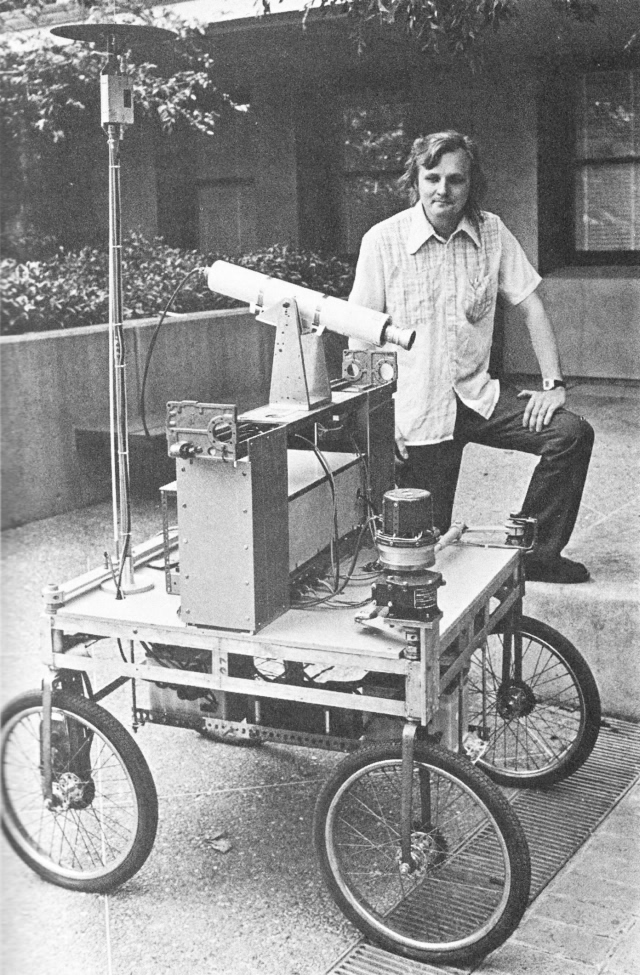
\includegraphics [scale=0.4] {stanford_cart}
  \caption{<<Стэнфордская тележка>>}
  \label{img:stanford_cart}
\end{figure}

В 1979 году Ханс Моравек перестраивает Стэнфордскую тележку, оснащая ее более
мощной системой технического зрения, и предпринимает ряд экспериментов по
трехмерному картографированию окружающей среды.

% Скопировано отсюда:
% http://www.lookatme.ru/mag/live/future-research/207541-sravnitelnaya-evolyutsiya-kak-razvivalis-roboty-i-chelovek

% Другие ссылки по теме:
% http://blog.skillfactory.ru/nauka-o-dannyh-data-science/vvedenie-v-mashinnoe-obuchenie/
% http://gagadget.com/science/21853-kak-razvivalis-bespilotnyie-avtomobili/
% https://strangernn.livejournal.com/1576029.html


%\newpage
%============================================================================================================================

\section{Aвтономный автомобиль Эрнста Дикманса} \label{sect_Dickmanns}

По сообщениям независимых экспертов первый полностью автономный автомобиль
был создан группой немецких ученных во главе с пионером робототехники
Эрнстом Дикмансом в 1980 году \cite{Dickmanns_vision}.
Для вычислений использовался мощный компьютер, который в то время был способен
уместиться лишь в грузовой фургон (рисунок \ref{img:dickmanns_car}).

\begin{figure}[ht] 
  \centering
  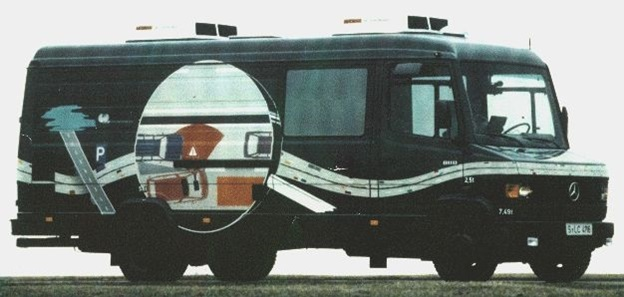
\includegraphics [scale=1.0] {dickmanns_car}
  \caption{Aвтономный автомобиль Эрнста Дикманса}
  \label{img:dickmanns_car}
\end{figure}

По данному проекту Дикмансом было опубликовано несколько научных работ, в 
которых детально описывались все технологии, применяемые в робомобиле. К ним 
можно отнести так называемый фильтр Калмана, имитацию саккадического движения 
глаз и механизмы параллельных вычислений. В некотором смысле эти технологии 
представляли собой модель машинного обучения, способную качественно оценивать 
всю окружающую обстановку.

% Скопировано отсюда:
% http://gagadget.com/science/21853-kak-razvivalis-bespilotnyie-avtomobili/

% Другие ссылки по теме:
% http://bespilot.com/info/istoriya
% https://geektimes.ru/post/274588/
% http://www.technoplusblog.ru/2017/10/blog-post.html


%\newpage
%============================================================================================================================

\section{Проект <<Прометей>>} \label{sect_Prometheus}

Автоконцерн Daimler-Benz обратил пристальное внимание на разработки Дикманса 
и запустил проект <<Прометей>>, основной целью которого было усовершенствование 
беспилотников и достижение беспрецедентной безопасности на дорогах. Проект 
взял старт в 1987 году и за время его существования (8 лет) было потрачено 
больше 1 млрд долларов \cite{MADI_GAZ}. <<Прометей>> вошел в историю как 
самый дорогой проект в сфере разработок робокаров ХХ века.
Однако инвестиции были потрачены не зря.

К середине 90-х миру были представлены два роботизированных беспилотника - 
VaMP (рисунок \ref{img:prometheus_vamp}) и VITA-2
(рисунок \ref{img:prometheus_vita2}). Они прошли успешное тестирование на 
полигоне в области Парижа, в процессе которого:

\begin{itemize}
  \item передвигались со скоростью до 130 км/ч полностью на автопилоте;
  \item самостоятельно перестраивались и меняли ряд;
  \item следили за дистанцией и передвижением других участников движения;
  \item обгоняли впереди идущие машины.
\end{itemize}

\begin{figure}[ht]
  {\centering
      \hfill
      \subbottom[List-of-Figures entry][VaMP\label{img:prometheus_vamp}]{%
          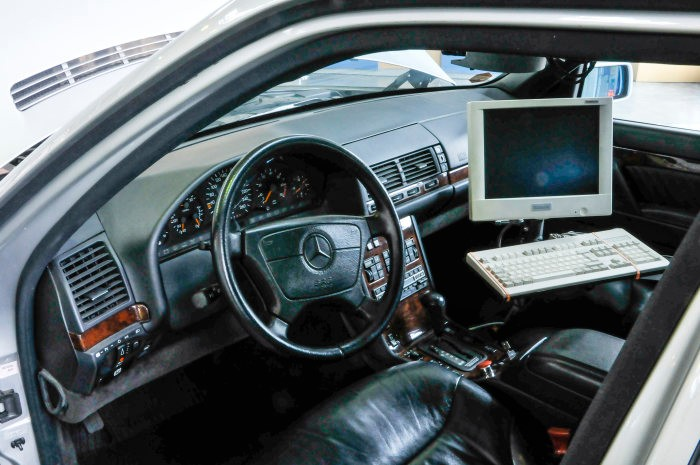
\includegraphics[width=0.44\linewidth]{prometheus_vamp}}
      \hfill
      \subbottom[VITA-2\label{img:prometheus_vita2}]{%
          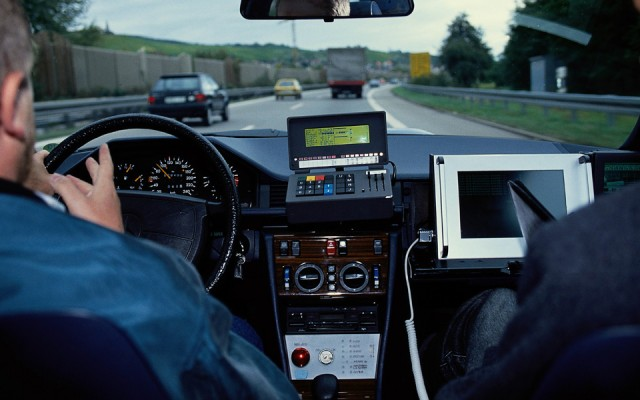
\includegraphics[width=0.47\linewidth]{prometheus_vita2}}
      \hfill
  }
  \caption{Автомобили проекта <<Прометей>>}
  \label{img:prometheus}
\end{figure}

Результатами проекта <<Прометей>> и разработками Дикманса воспользовались для 
серийного производства Mersedes-ов S-класса 1995 года. Эти машины были 
оснащены более продвинутой системой круиз-контроля, которая позволяла 
адаптироваться к средней скорости автомобильного потока и не нарушать дистанцию 
между авто.

% Скопировано отсюда:
% http://bespilot.com/info/istoriya

% Другие ссылки по теме:
% http://gagadget.com/science/21853-kak-razvivalis-bespilotnyie-avtomobili/
% https://geektimes.ru/post/274588/
% http://www.technoplusblog.ru/2017/10/blog-post.html


%\newpage
%============================================================================================================================

\section{Соревнования DARPA} \label{sect_DARPA}

В 2001 году американское агентство DARPA (Defense Advanced Research Projects 
Agency — агентство перспективных исследовательских проектов для нужд обороны) 
занялось проектом по созданию беспилотного автомобиля, который способен без 
участия человека прокладывать маршрут и двигаться к заданной точке, 
преодолевая встречающиеся на пути препятствия \cite{DARPAchallnge}.
К реализации этого проекта, 
финансируемого Министерством обороны США, привлечено множество коллективов 
разработчиков из различных компаний, высших учебных заведений и академических 
институтов. Руководители американского оборонного ведомства рассчитывают на 
то, что к 2015 году каждое третье наземное транспортное средство американских 
ВС станет беспилотным.

Для оценки достигнутых успехов, а также поощрения коллективов, представивших 
самые передовые разработки в данной области, DARPA организует специальные 
соревнования для беспилотных автомобилей (рисунок \ref{img:darpa_3cars}).
Первый турнир DARPA Grand Challenge 
2004 прошел 13 марта 2004 года. За главный приз (1 млн долл.) боролись 
автомобили полутора десятков команд.

\begin{figure}[ht] 
  \centering
  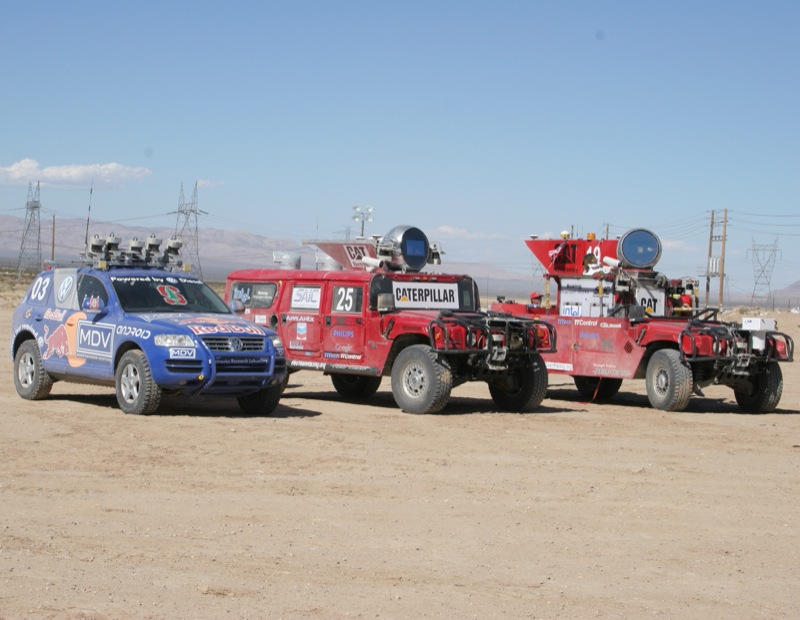
\includegraphics [scale=0.5] {darpa_3cars}
  \caption{Беспилотные автомобили DARPA Grand Challenge}
  \label{img:darpa_3cars}
\end{figure}

Маршрут протяженностью 230 км был проложен в основном по пустыне от города 
Барстоу (шт. Калифорния) до Приммы (шт. Невада). Организаторы соревнований 
не ограничивали размер и вес автомобилей. При этом было запрещено участие 
какого-либо живого существа в процессе управления транспортным средством. 
Кроме того, роботизированные автомобили не должны были наносить повреждения 
другим транспортным средствам, дорожному покрытию и природным объектам.
% ---
Точную информацию о маршруте представителям команд передали лишь за 2 часа до 
старта. Задача усложнялась еще и тем, что трасса не везде проходила по дорогам, 
а на пути автомобилей попадались различные естественные и искусственные 
препятствия: канавы, глубокие колеи в грунте, песчаные участки, лужи, камни, 
тоннели и пр.

Стартовать в DARPA Grand Challenge 2004 смогли восемь автомобилей, однако до 
финиша ни один из претендентов не добрался. Лучшему из участников удалось 
преодолеть лишь около 12 км.
% ---
8 октября 2005-го, состоялся финальный заезд 
DARPA Grand Challenge 2005. Маршрут протяженностью почти 212~км был проложен 
по каменистой пустыне Мохава. На преодоление дистанции участникам было отведено 
не более 10 ч. Призовая сумма за победу в состязании составила 2~млн~долл.

В ходе предварительных заездов из 195 автомобилей-роботов были отобраны 23 
финалиста. Четыре из них сумели добраться до финиша в течение отведенного 
времени, что, несомненно, стало свидетельством значительного прогресса, 
которого удалось добиться разработчикам роботов. Победил автомобиль Stanley, 
показанный на рисунке \ref{img:darpa_2005winner}, созданный на базе серийного 
VW Touareg сотрудниками команды Stanford Racing 
Team из Стэнфордского университета. Stanley смог самостоятельно преодолеть 
212~км по пустыне и выйти в конечную точку заданного маршрута
за 6~ч~53~мин~58~с. Средняя скорость передвижения составила около 30 км/ч.

\begin{figure}[ht] 
  \centering
  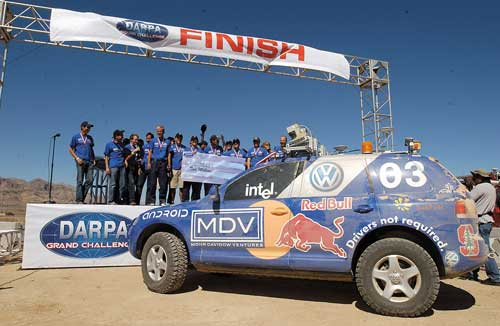
\includegraphics [scale=0.8] {darpa_2005winner}
  \caption{Победитель DARPA Grand Challenge 2005}
  \label{img:darpa_2005winner}
\end{figure}

Следующие соревнования прошли в конце 2007 года. На этот раз организаторы 
усложнили задачу. Автомобилям-роботам предстояло ездить не по пустыне, а по 
городским улицам среди множества других транспортных средств, соблюдая правила 
дорожного движения штата Калифорния и учитывая требования дорожных знаков и 
разметки. Кардинальные изменения регламента были отражены и в названии турнира, 
переименованного в DARPA Urban Challenge. Призовая сумма за первое место 
составила 2 млн долл., за второе — 1 млн и за третье — 500 тыс.

Местом проведения состязания был выбран тренировочный полигон на территории 
бывшей базы ВВС США, расположенный в Викторвилле (Victorville) в штате 
Калифорния. В настоящее время этот полигон используется подразделениями 
армии США для отработки проведения военных операций в городских условиях.

По итогам региональных квалификационных заездов было отобрано 35 команд, 
получивших право участвовать в национальном квалификационном туре 
(National Qualification Event, NQE). В течение восьми дней команды, допущенные 
к участию в NQE, тщательно тестировали свои беспилотные транспортные средства 
в условиях городского движения. Помимо роботов по дорогам ездили и обычные 
автомобили, управляемые людьми. Квалификационные задания включали движение в 
потоке других транспортных средств, проезд перекрестков разных типов и развязок 
с круговым движением, объезд препятствий, парковку и пр.

По итогам NQE организаторы соревнований отобрали 11 команд для участия в 
финальном заезде DARPA Urban Challenge 2007 представленных 
на рисунке \ref{img:darpa_urban}. Заезд состоялся 3 ноября 2007 
года. Каждому из участников необходимо было доставить груз в заданную точку, 
пройдя около 100 км через промежуточные контрольные точки (их координаты были 
предоставлены командам незадолго до старта) и уложившись в шестичасовой лимит. 
Во время проведения соревнований по улицам полигона, помимо роботов, двигалось 
более 50 автомобилей, имитирующих городской трафик. За нарушения ПДД 
начислялись штрафные баллы, а столкновение с другим участником движения или 
препятствием каралось дисквалификацией.

\begin{figure}[ht] 
  \centering
  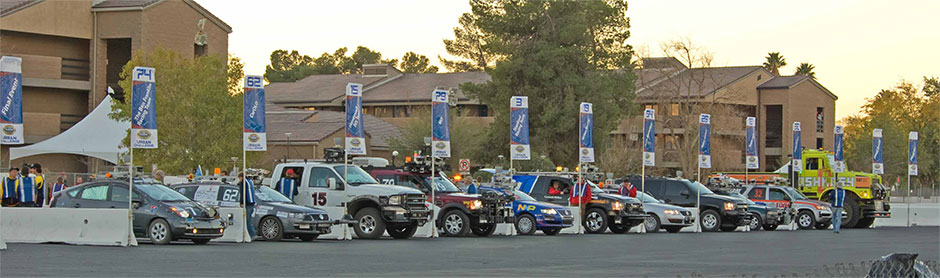
\includegraphics [scale=0.5] {darpa_urban}
  \caption{Старт DARPA Urban Challenge 2007}
  \label{img:darpa_urban}
\end{figure}

Ожидания тех, кто жаждал увидеть многочисленные аварии автомобилей-роботов, 
не оправдались. Впрочем, небольшие инциденты все-таки происходили. Примерно 
через час после старта в системе управления беспилотного грузовика команды 
Oshkosh возникли неполадки, и его остановили во избежание столкновения с 
одним из зданий полигона. Примерно за час до истечения лимита времени, 
отпущенного на выполнение задания, произошло столкновение двух 
автомобилей-роботов, которые не получили серьезных повреждений 
(скорость в момент контакта была небольшая), однако, согласно правилам 
соревнования, были дисквалифицированы. Тем не менее по сравнению с турнирами 
2004 и 2005 годов прогресс налицо — особенно с учетом того обстоятельства, что 
участникам DARPA Urban Challenge 2007 пришлось решать более сложные задачи.

% Скопировано отсюда:
% https://compress.ru/article.aspx?id=19754

% Другие ссылки по теме:
% http://www.thg.ru/game/20050206/index.html
% https://3dnews.ru/167147
% http://www.membrana.ru/particle/2661


%\newpage
%============================================================================================================================

\section{Беспилотный автомобиль Google} \label{sect_Google}

В 2008 году в Google серьезно задумались над решением проблем на дорогах и привлекли 
разработчиков из команды Stanley, победившей DARPA Grand Challenge во главе с 
профессором Себастьяном Труном.

Ответом на сложный вопрос в итоге должен стать полностью автономный 
автомобиль, по задумке способный уверенно и безопасно передвигаться по дорогам, 
всегда действовать по правилам, но делать это плавно, чтобы обеспечить комфорт 
пассажиров, при этом отнимая у них возможность управлять движением. К 2009 году 
в Google собрали опытную команду инженеров, и практическая работа над проектом 
началась. 

Для реализации поставленной задачи разработчики используют лазерные датчики, 
видеокамеры, радары и GPS (рисунок \ref{img:google_car_scheme}). 
Данная система технического зрения способна анализировать ситуацию, 
определять объекты, препятствия и дорожные знаки вокруг, прогнозировать 
ситуацию и полностью контролировать автомобиль \cite{MADI_GAZ}.

\begin{figure}[ht] 
  \centering
  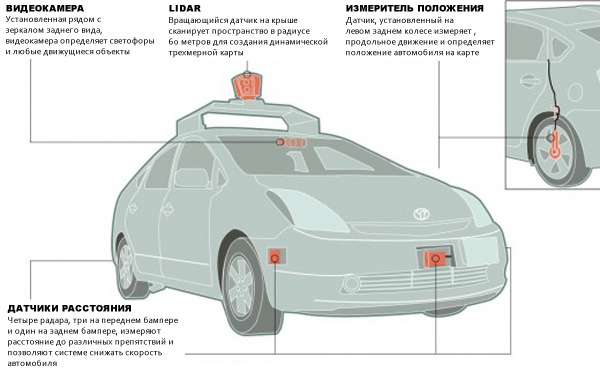
\includegraphics [scale=0.8] {google_car_scheme}
  \caption{Техническое зрение беспилотного автомобиля Google}
  \label{img:google_car_scheme}
\end{figure}

Google оснастила группу из десяти автомобилей, включая три гибридных 
Lexus RX450h, одну Audi TT и шесть Toyota Prius дополнительным технологическим 
оборудованием. Выбор этих моделей серийных автомобилей был не случаен. 
Рассматривались машины с изначально высокой степенью интеграции электронных 
систем управления.

Была проведена серия испытаний с экспертом-водителем, который сидел на 
водительском сидении и инженерами Google на пассажирских сидениях. 
Испытания проводились в местах с различным ландшафтом и интенсивностью 
автомобильного движения на территории США.

Ограничения скоростных режимов были сохранены в памяти систем управления и в 
случае нештатной ситуации всегда была возможность перейти на ручное управление 
автомобилем. В августе 2012 года, Google объявила, что завершено полмиллиона 
миль дорожных испытаний. По состоянию на декабрь 2013 года, четыре штата в 
США — Калифорния, Флорида, Невада и Мичиган, приняли законы, позволяющие 
использование самоуправляемых автомобилей.

% Скопировано отсюда:
% https://vc.ru/10704-apple-google-car
% http://robotosha.ru/robotics/how-it-works-driverless-car-google.html

